\documentclass[11pt,twocolumn,oneside,openany,headings=optiontotoc,11pt,numbers=noenddot,final]{article}

\usepackage[a4paper]{geometry}
\usepackage[utf8]{inputenc}
\usepackage[T1]{fontenc}
\usepackage{lmodern}
\usepackage[ngerman]{babel}
\usepackage{ngerman}

\usepackage[onehalfspacing]{setspace}

\usepackage{fancyhdr}
\usepackage{fancybox}

\usepackage{rotating}
\usepackage{varwidth}

%Struktogramme
\usepackage[german,curves]{struktex}

\usepackage{pdflscape}
\usepackage{changepage}
\usepackage{graphicx}
\usepackage[bottom]{footmisc}
\usepackage{transparent}
\usepackage{graphbox}
\graphicspath{
	{Pics/PDFs/}
	{Pics/JPGs/}
	{Pics/PNGs/}
}
\usepackage{caption}
\usepackage{wrapfig}
\usepackage{marginnote}
\usepackage{tabularx}
\usepackage{dashrule}
\usepackage{soulutf8}
\usepackage{hhline}
%arydshln suppresses vertical lines in table
%\usepackage{arydshln}
\usepackage{multirow}
\usepackage{enumerate}
\usepackage[hidelinks]{hyperref}
\usepackage{listings}

\usepackage[table]{xcolor}
\usepackage{array}
\usepackage{enumitem,amssymb,amsmath}
\usepackage{interval}
\usepackage{cancel}
\usepackage{stmaryrd}
\usepackage{wasysym}
\usepackage{polynom}
\usepackage{diagbox}
\usepackage{dashrule}
\usepackage{framed}
\usepackage{mdframed}
\usepackage{karnaugh-map}
\usepackage{pdfpages}

\usepackage{blindtext}

\usepackage{eso-pic}

\usepackage{amssymb}
\usepackage{eurosym}

\usepackage[pages=some]{background}
\pagestyle{headings}
\renewcommand{\headrulewidth}{0.2pt}
\renewcommand{\footrulewidth}{0.2pt}
\newcommand*{\underdownarrow}[2]{\ensuremath{\underset{\overset{\Big\downarrow}{#2}}{#1}}}
\setlength{\fboxsep}{5pt}
\newcommand{\explainBelow}[3]{\underbrace{#1}_{\parbox{\widthof{#3}}{\footnotesize\raggedright #2}}}
\newcommand{\explainAbove}[3]{\overbrace{#1}^{\parbox{\widthof{#3}}{\footnotesize\raggedright #2}}}
\newcommand\footnoteref[1]{\protected@xdef\@thefnmark{\ref{#1}}\@footnotemark}


% Codestyle defined
\definecolor{codegreen}{rgb}{0,0.6,0}
\definecolor{codegray}{rgb}{0.5,0.5,0.5}
\definecolor{codepurple}{rgb}{0.58,0,0.82}
\definecolor{backcolour}{rgb}{0.95,0.95,0.92}
\definecolor{deepgreen}{rgb}{0,0.5,0}
\definecolor{darkblue}{rgb}{0,0,0.65}
\definecolor{mauve}{rgb}{0.40, 0.19,0.28}
\colorlet{exceptioncolour}{yellow!50!red}
\colorlet{commandcolour}{blue!60!black}
\colorlet{numpycolour}{blue!60!green}
\colorlet{specmethodcolour}{violet}

%Neue Spaltendefinition
\newcolumntype{L}[1]{>{\raggedright\let\newline\\\arraybackslash\hspace{0pt}}m{#1}}
\newcolumntype{M}{>{\centering\arraybackslash}X}
\newcommand{\cmnt}[1]{\ignorespaces}
%Textausrichtung ändern
\newcommand\tabrotate[1]{\rotatebox{90}{\raggedright#1\hspace{\tabcolsep}}}

%Intervall-Konfig
\intervalconfig {
	soft open fences
}

%Bash
\lstdefinestyle{BashInputStyle}{
	language=bash,
	basicstyle=\small\sffamily,
	backgroundcolor=\color{backcolour},
	columns=fullflexible,
	backgroundcolor=\color{backcolour},
	breaklines=true,
}
%Java
\lstdefinestyle{JavaInputStyle}{
	language=Java,
	backgroundcolor=\color{backcolour},
	aboveskip=1mm,
	belowskip=1mm,
	showstringspaces=false,
	columns=flexible,
	basicstyle={\footnotesize\ttfamily},
	numberstyle={\tiny},
	numbers=none,
	keywordstyle=\color{purple},,
	commentstyle=\color{deepgreen},
	stringstyle=\color{blue},
	emph={out},
	emphstyle=\color{darkblue},
	emph={[2]rand},
	emphstyle=[2]\color{specmethodcolour},
	breaklines=true,
	breakatwhitespace=true,
	tabsize=2,
}
%Python
\lstdefinestyle{PythonInputStyle}{
	language=Python,
	alsoletter={1234567890},
	aboveskip=1ex,
	basicstyle=\footnotesize,
	breaklines=true,
	breakatwhitespace= true,
	backgroundcolor=\color{backcolour},
	commentstyle=\color{red},
	otherkeywords={\ , \}, \{, \&,\|},
	emph={and,break,class,continue,def,yield,del,elif,else,%
		except,exec,finally,for,from,global,if,import,in,%
		lambda,not,or,pass,print,raise,return,try,while,assert},
	emphstyle=\color{exceptioncolour},
	emph={[2]True,False,None,min},
	emphstyle=[2]\color{specmethodcolour},
	emph={[3]object,type,isinstance,copy,deepcopy,zip,enumerate,reversed,list,len,dict,tuple,xrange,append,execfile,real,imag,reduce,str,repr},
	emphstyle=[3]\color{commandcolour},
	emph={[4]ode, fsolve, sqrt, exp, sin, cos, arccos, pi,  array, norm, solve, dot, arange, , isscalar, max, sum, flatten, shape, reshape, find, any, all, abs, plot, linspace, legend, quad, polyval,polyfit, hstack, concatenate,vstack,column_stack,empty,zeros,ones,rand,vander,grid,pcolor,eig,eigs,eigvals,svd,qr,tan,det,logspace,roll,mean,cumsum,cumprod,diff,vectorize,lstsq,cla,eye,xlabel,ylabel,squeeze},
	emphstyle=[4]\color{numpycolour},
	emph={[5]__init__,__add__,__mul__,__div__,__sub__,__call__,__getitem__,__setitem__,__eq__,__ne__,__nonzero__,__rmul__,__radd__,__repr__,__str__,__get__,__truediv__,__pow__,__name__,__future__,__all__},
	emphstyle=[5]\color{specmethodcolour},
	emph={[6]assert,range,yield},
	emphstyle=[6]\color{specmethodcolour}\bfseries,
	emph={[7]Exception,NameError,IndexError,SyntaxError,TypeError,ValueError,OverflowError,ZeroDivisionError,KeyboardInterrupt},
	emphstyle=[7]\color{specmethodcolour}\bfseries,
	emph={[8]taster,send,sendMail,capture,check,noMsg,go,move,switch,humTem,ventilate,buzz},
	emphstyle=[8]\color{blue},
	keywordstyle=\color{blue}\bfseries,
	rulecolor=\color{black!40},
	showstringspaces=false,
	stringstyle=\color{deepgreen}
}

\lstset{literate=%
	{Ö}{{\"O}}1
	{Ä}{{\"A}}1
	{Ü}{{\"U}}1
	{ß}{{\ss}}1
	{ü}{{\"u}}1
	{ä}{{\"a}}1
	{ö}{{\"o}}1
}

% Neue Klassenarbeits-Umgebung
\newenvironment{worksheet}[3]
% Begin-Bereich
{
	\newpage
	\sffamily
	\setcounter{page}{1}
	\ClearShipoutPicture
	\AddToShipoutPicture{
		\put(55,761){{
				\mbox{\parbox{385\unitlength}{\tiny \color{codegray}BBS I Mainz, #1 \newline #2
						\newline #3
					}
				}
			}
		}
		\put(455,761){{
				\mbox{\hspace{0.3cm}
\includegraphics[width=0.2\textwidth]{../../logo.pdf}}
			}
		}
	}
}
% End-Bereich
{
	\clearpage
	\ClearShipoutPicture
}

\setlength{\columnsep}{3em}
\setlength{\columnseprule}{0.5pt}

\geometry{left=2.50cm,right=2.50cm,top=3.00cm,bottom=1.00cm,includeheadfoot}
\pagenumbering{gobble}
\pagestyle{empty}

\begin{document}
	\begin{worksheet}{HBF IT 17A}{Grundstufe}{Lernbaustein 3 - LB 2: Einführung in die Differentialrechnung}
		\section{Worum geht es in der Differentialrechnung?}
		Abgesehen von dem absoluten Wert für eine Größe ist auch die Tendenz dieser Größe, mit der Sie sich verändert, interessant.\\
		Die erste Sequenz versucht daher, ihnen eine erste Vorstellung zum Begriff der \glqq{}Ableitung\grqq{} zu vermitteln. Deren Verständnis ist für die nachfolgende Mathematik relevant.
		\subsection*{Beispiel 1: Bevölkerung der BRD und Indien}
		Die Bevölkerung der BRD beträgt knapp 82 Mio. Die Bevölkerung Indiens beträgt ungefähr 1,1 Mrd.\\
		\par
		Neben unterschiedlichen absolute Werten weisen die Bevölkerungswerte auch unterschiedliche Wachstumstendenzen zum jetzigen Zeitpunkt auf. Das geht aus der Darstellung der vergangenen und zukünftigen Entwicklung hervor:\\
		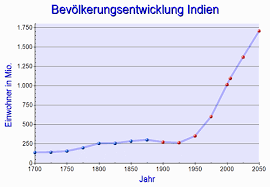
\includegraphics[scale=0.8]{Bilder/BevIndien.png}\\
		\par
		\noindent
		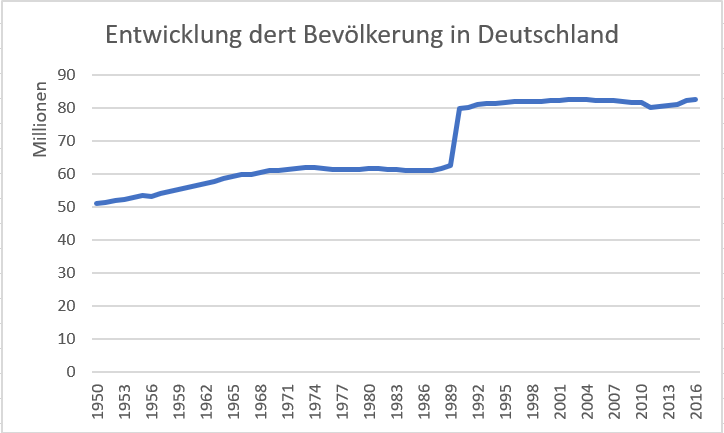
\includegraphics[scale=0.59]{Bilder/BevDeutschland.png}
		\tiny{Bis 1989: Früheres Bundesgebiet}
		\normalsize
		\subsection*{Beispiel 2: Schulden in Deutschland}
		Neben den absoluten Schuldenwerten ändert sich auch die Wachstumstendenz. So kann man hier erkennen, dass 1990 eine andere Dynamik vorlag als 2010.
		\begin{table}[htb]
			\begin{tabularx}{0.5\textwidth}{|X|X|}
				\hline
				Jahr (0=1990; in Jahren) & Schuldenstand in Milliarden\\
				\hline
				0 & 600\\
				\hline
				5 & 1.018\\
				\hline
				10 & 1.210\\
				\hline
				15 & 1.489\\
				\hline
				20 & 2.011\\
				\hline
				25 & 2.000\\
				\hline
			\end{tabularx}
		\end{table}
		\section{Die \underline{durchschnittliche} Änderungsrate \underline{über einem Intervall [\(x_{0};x_{1}\)]}}
		Die durchschnittliche Änderungsrate über einem Intervall ist eine Maßzahl für die Dynamik in einem Zeitraum / in einem Intervall. Sie ist der Quotient aus dem absoluten Zuwachs in einem Intervall der Länge des Intervalls.\\
		\par\noindent
		Graphisch lässt sich dieser Wert als Steigung einer Sekante an den Punkten P (\(x_{0}\) | f(\(x_{0}\))) und Q (\(x_{1}\) | f(\(x_{1}\))) interpretieren.
		\subsection{Übungen}
		\begin{enumerate}
			\item Berechnen Sie die durchschnittliche Änderungsraten zu den im ersten Kapitel gegebenen Entwicklungen zu den folgenden Intervallen:
			\begin{itemize}
				\item[(a)] Bevölkerungsentwicklung Indien: [2010;2050]\\
				Bevölkerungsentwicklung Deutschland: [2010;2050]\\
				Bevölkerungsentwicklung Deutschland: [2010;2040]\\
				Bevölkerungsentwicklung Deutschland: [2010;2020]\\
				Bevölkerungsentwicklung Deutschland: [2010;2011]\\
				\item[(b)] Welche der zu Deutschland berechneten Wachstumsraten ist am besten geeignet, die \underline{momentane} Wachstumsdynamik zum Zeitpunkt 2010 zum Ausdruck zu bringen?
			\end{itemize}
			\item Stellen Sie die Änderung der Schuldendynamik in Deutschland in einer Form ihrer Wahl dar!
		\end{enumerate}
		\section{Von der \underline{durchschnittlichen} Änderungsrate zur \underline{momentanen} Änderungsrate}
		Die durchschnittliche Änderungsrate ist nur eine Annäherung an die Dynamik an einer bestimmten Stelle. Da sich die Dynamik schnell ändern kann, ist häufig die Dynamik zu einem bestimmten Zeit\underline{punkt} relevant.
		\subsubsection*{Beispiel 1: Radarkontrolle}
		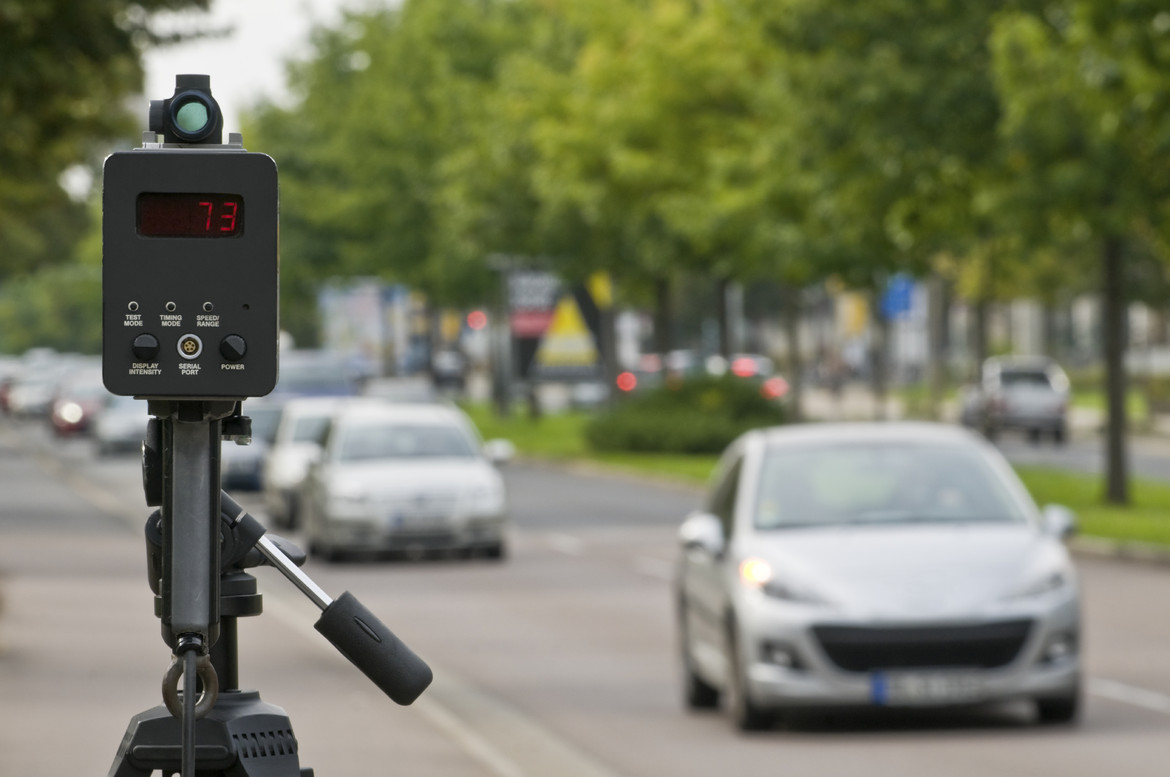
\includegraphics[scale=0.6]{Bilder/radar.jpg}
		\subsubsection*{Beispiel 2: Fallschirmsprung}
		Nach 2 Sekunden hat der Fallschirmspringer schon eine Geschwindigkeit von\\
		\begin{center}
			\fbox{???} km/h
		\end{center}
		erreicht?\\
		\par\noindent
		
		\subsection{Die Bestimmung der \underline{momentanen} Änderungsrate \underline{an einer Stelle \(x_{0}\)}}
		Die durchschnittliche Änderungsrate kann nur ein ungefähres Bild der tatsächlichen Dynamik bzw. Steigung an einem bestimmten Punkt liefern Je größer das Intervall ist, für den die Dynamik betrachtet wird, umso schlechter wird in der Regel die Realität dargestellt.\\
		\par\noindent
		Daher können wir versuchen, die Steigung in einem Punkt anzunähern, indem wir das Intervall, für welches wir die Dynamik betrachten, immer kleiner werden lassen.\\
		\par\noindent
		Im Gegensatz zur durchschnittlichen Änderungsrate, die die Dynamik über einem Intervall beschreibt, gibt die \textbf{momentane Änderungsrate} die Dynamik in einem bestimmten Punkt wieder.
		\subsubsection*{\underline{Die Idee}}
		Wir benennen das Intervall [\(x_{0};x_{1}\)] mit \(h\) und lassen dieses beliebig klein werden.
		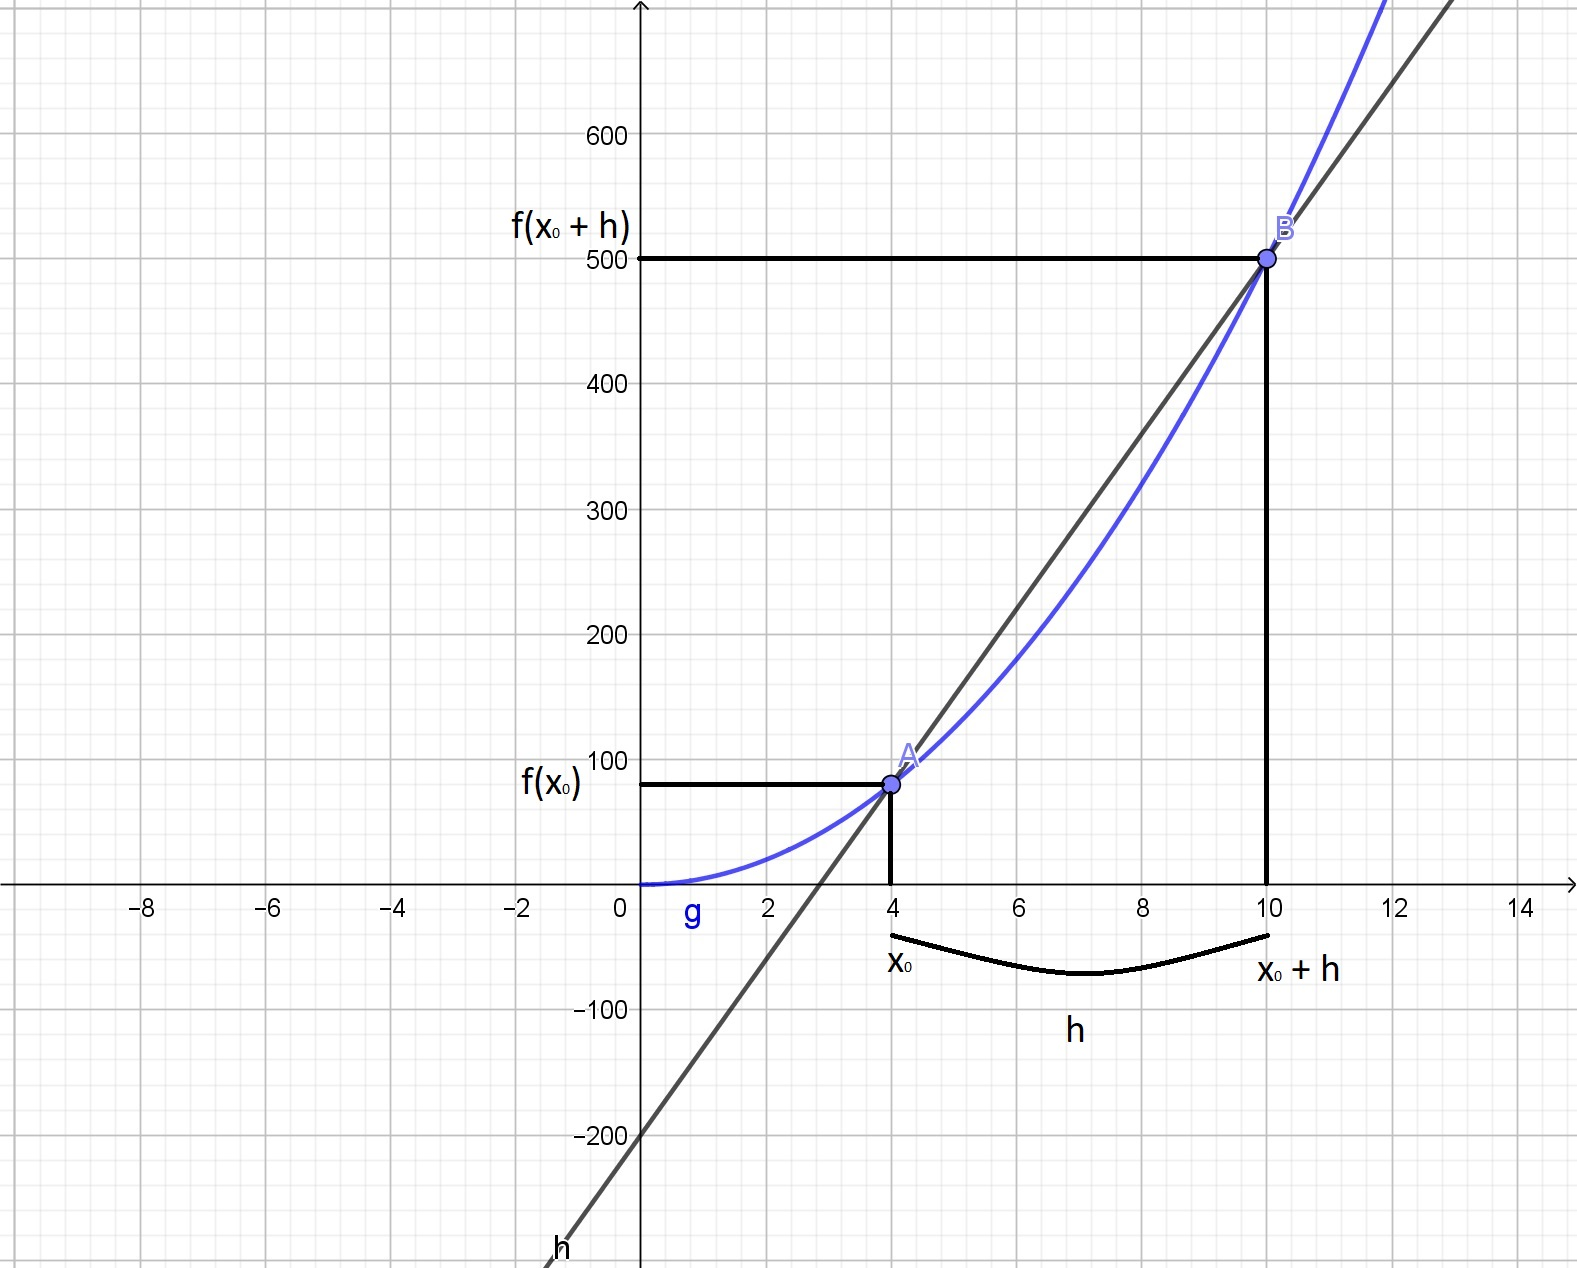
\includegraphics[scale=0.25]{Bilder/DifferenzenquotienthMeth.jpg}
		Die Sekante hat nun die Steigung:\\
		\begin{center}
			\(m_{[x_{0},x_{0}+h]} = \frac{f(x_{0}+h) - f(x_{0})}{h}\)
		\end{center}
		\subsubsection*{\underline{Ihre Aufgabe:}}
		Berechnen Sie für die folgenden Funktionen die mittlere Änderungsrate im Intervall \textit{I}.
		\begin{itemize}
			\itemsep0pt
		\item[(a)] \(f(x) = 3x^{2} \text{ im Intervall } I=[0;4]\)
			\item[(b)] \(f(x) = -2x^{3} + 2 \text{ im Intervall } I=[1;5]\)
		\end{itemize}
	\end{worksheet}
\end{document}